\section{异能态对波函数的选择}\label{sec:4-6}

在第2.3节中，我们建立了 BCS 配对理论与准粒子真空的微观表象；在第2.5节中，推演了内禀参考系的对称性破缺、角动量投影及欧拉角定向；在第2.7节中，确立了截断模型空间中有效电磁跃迁算符的幺正重整化规范；在第5.9节中，给出了由激发态绝对寿命 $\tau$、光子分支比与内转换系数反演约化跃迁几率 $B(\sigma L)$ 的严格测量模型。在低能核物理与在束 $\gamma$ 谱学研究中，寿命长于约数纳秒至数毫秒乃至数年的核能级被称为同核异能态（Nuclear Isomers）~\cite{book-jain-nuclear-isomers,walker-1999-nature-nuclear-isomers}。

这引出了本节的核心科学问题：\textbf{长寿命同核异能态究竟对多体波函数的特定微观成分施加了何种选择性约束？异能态的产生为什么不能归结为单一的微观原因？}

从电磁跃迁辐射场量子理论出发，从初态向末态发射多极度为 $L$ 的单光子跃迁发射率满足基础标度关系：
\begin{equation}\label{eq:4-6-rate-scaling}
\lambda_\gamma(\sigma L) \propto \left(\frac{E_\gamma}{\hbar c}\right)^{2L + 1} B(\sigma L; I_i \to I_f).
\end{equation}
激发态呈现出长寿命（即辐射跃迁速率 $\lambda_\gamma$ 极小），在微观上可由以下四个截然不同的物理机制或其相干叠加所导致：
\begin{enumerate}
\item \textbf{自旋陷阱（Spin Traps）：} 纯运动学与电磁场相空间压制。初末态总角动量差极大（$L \ge 4$）而衰变激发能 $E_\gamma$ 极小，相空间因子 $(E_\gamma/\hbar c)^{2L+1}$ 使跃迁速率受到极强压制。
\item \textbf{Seniority 异能态：} 微观多体矩阵元结构相消。在球形或近球形单 $j$ 壳层同种核子体系中，配对相互作用的准自旋几何对称性导致半满壳处 $\Delta v = 0$ 的电四极跃迁矩阵元严格为零：$B(E2) \to 0$。
\item \textbf{K 异能态：} 空间取向与转动投影阻碍。在轴对称强变形核中，微观组态在对称轴上的总角动量投影量子数改变量超过光子多极度（$\Delta K > L$），跃迁受制于极微弱的禁戒杂化振幅。
\item \textbf{形状异能态（Shape Isomers）：} 空间构型重叠与位垒隧穿压制。斯楚廷斯基（Strutinsky）双峰裂变位垒使原子核俘获在超形变第二极小（如锕系区 $\beta_2 \approx 0.6$），其波函数与正常形变第一极小基态波函数在集体坐标空间被内位垒隔离，WKB 隧穿穿透几率极低。
\end{enumerate}
在实际原子核中，上述机制可同时并存（例如高自旋自旋陷阱同时叠合 $K$ 禁戒）。关于绝对跃迁几率的带量纲换算常数、内转换系数 $\alpha_{\mathrm{IC}}$ 及分支比提取模型，统一对齐至第5.9节。本节重点推导单 $j$ 壳层准自旋 $SU(2)$ 代数及其半满壳相消定理，建立轴对称 $K$ 禁戒度幂律标度 $f_\nu$，剖析三轴非轴对称形变引入 $K$ 混合后阻碍度依然存在的微观动力学，并阐明超形变形状异能态的位垒选择。

\subsection{单 j 壳层准自旋代数与 Seniority 半满壳相消}\label{sec:4-6-1}

考虑由同种核子（纯质子或纯中子）占据的一个孤立单粒子轨道 $j$。定义该单粒子轨道的\textbf{对简并度}（Pair Degeneracy）为：
\begin{equation}\label{eq:4-6-pair-degeneracy}
\Omega_j \equiv \frac{2j + 1}{2}.
\end{equation}
在此特别声明：$\Omega_j$ 为单个单粒子轨道允许容纳的时间反演核子对的最大数目（如 $j=11/2$ 时 $\Omega_j = 6$），切勿与欧拉角定向 $\Omega = (\phi, \theta, \psi)$ 或部分文献中定义的全壳单核子容纳数 $2j+1$ 混淆。

设粒子数算符为 $\hat{N} = \sum_{m=-j}^j c_{jm}^\dagger c_{jm}$，核子总数为 $n$。Seniority 量子数 $v$ 定义为\textbf{纯单 $j$ 壳层中未配对核子数}（亦即在纯配对哈密顿量本征基底下的未成对准自旋标签），它专门刻画未凝聚为零角动量对（$J=0$）的核子自由度，与一般形变或多道微观场中的 BCS 准粒子数具有不同的数学范畴。第2.3节中的 $P_k^\dagger = c_k^\dagger c_{\bar{k}}^\dagger$ 指代单个时间反演单粒子对算符；在此处的单 $j$ 壳层中，全壳归一化集体对算符定义为对所有磁子态 $m>0$ 的相干求和 $\hat{P}_{\mathrm{coll}}^\dagger \equiv \frac{1}{\sqrt{\Omega_j}} \sum_{m>0} (-1)^{j-m} c_{jm}^\dagger c_{j,-m}^\dagger = \frac{1}{\sqrt{\Omega_j}} \sum_{k>0} P_k^\dagger$。在此基础上定义准自旋升阶、降阶与第三分量算符满足 $\hat{S}_+ = \sqrt{\Omega_j} \hat{P}_{\mathrm{coll}}^\dagger = \sum_{k>0} P_k^\dagger$~\cite{book-jain-nuclear-isomers}：
\begin{align}
\hat{S}_+ &\equiv \sum_{m>0} (-1)^{j-m} c_{jm}^\dagger c_{j,-m}^\dagger = \sqrt{\Omega_j} \hat{P}^\dagger, \label{eq:4-6-Splus-def}\\
\hat{S}_- &\equiv (\hat{S}_+)^\dagger = \sum_{m>0} (-1)^{j-m} c_{j,-m} c_{jm}, \label{eq:4-6-Sminus-def}\\
\hat{S}_0 &\equiv \frac{1}{2} \left( \hat{N} - \Omega_j \right) = \frac{n - \Omega_j}{2}. \label{eq:4-6-Szero-def}
\end{align}
利用费米子反对易关系，直接计算对易子：
\begin{equation}\label{eq:4-6-quasispin-commutation}
[\hat{S}_+, \hat{S}_-] = 2 \hat{S}_0, \quad [\hat{S}_0, \hat{S}_\pm] = \pm \hat{S}_\pm.
\end{equation}
式~\eqref{eq:4-6-quasispin-commutation} 表明，算符组 $\{\hat{S}_+, \hat{S}_-, \hat{S}_0\}$ 在准自旋空间构成严格的李代数 $SU(2)$。准自旋 Casimir 算符为 $\hat{\mathbf{S}}^2 = \hat{S}_+ \hat{S}_- + \hat{S}_0(\hat{S}_0 - 1)$。

多粒子态矢 $|j^n v \alpha J M\rangle$ 对应于准自旋本征态 $|S, S_0; v \alpha J M\rangle$（其中 $\alpha$ 为区分具有相同 $v, J$ 的附加简并度标签，在以下同一多重态的代数推导中保持固定）。当体系中仅有 $v$ 个未配对核子且不存在任何 $J=0$ 对时（即 $n = v$ 基底状态），该状态必被降阶算符消除：$\hat{S}_- |j^v v \alpha J M\rangle = 0$。因此 $n=v$ 态对应于准自旋多重态的最低投影态 $S_0 = -S$：
\begin{equation}\label{eq:4-6-quasispin-quantum-number}
S_0(n=v) = \frac{v - \Omega_j}{2} = -S \implies S = \frac{\Omega_j - v}{2}, \quad S_0 = \frac{n - \Omega_j}{2}.
\end{equation}
由此可见，Seniority $v$ 严格等价于总准自旋的大小 $S$，而粒子数 $n$ 则直接对应准自旋的第三分量投影 $S_0$。

现在考虑电磁多极跃迁算符在准自旋空间中的张量性质。在第二量子化下，单粒子电磁多极算符写作：
\begin{equation}\label{eq:4-6-EM-operator-second-quant}
\hat{\mathcal{M}}(\sigma L, M) = \sum_{m_1, m_2} \langle j m_1 | \hat{\mathcal{M}} | j m_2 \rangle c_{jm_1}^\dagger c_{jm_2}.
\end{equation}
在粒子-空穴变换（$c_{jm}^\dagger \leftrightarrow (-1)^{j-m} c_{j,-m}$）下，对于多极度 $L > 0$ 且为偶数的单体电算符（特别是电四极跃迁算符 $E2$），算符在粒子-空穴对置下改变符号。在准自旋空间中，它严格表现为一个\textbf{秩为 $s=1$、第三分量为 $s_0=0$ 的准自旋矢量算符}：
\begin{equation}\label{eq:4-6-operator-quasispin-tensor}
\hat{T}^{(s=1, s_0=0)}_{LM} = \hat{\mathcal{M}}(EL, M) \quad (L > 0, \text{偶数}).
\end{equation}

对准自旋空间应用 Wigner-Eckart 定理，考虑相同 Seniority 态之间的跃迁（$\Delta v = 0$，即初末态具有相同的总准自旋 $S = \frac{\Omega_j - v}{2}$）：
\begin{equation}\label{eq:4-6-quasispin-wigner-eckart}
\langle S, S_0, v J_f || \hat{\mathcal{M}}(E2) || S, S_0, v J_i \rangle = \frac{C_{S S_0 1 0}^{S S_0}}{C_{S (-S) 1 0}^{S (-S)}} \langle S, (-S), v J_f || \hat{\mathcal{M}}(E2) || S, (-S), v J_i \rangle,
\end{equation}
其中分母对应 $n=v$ 时的基底矩阵元。查阅 Clebsch-Gordan 系数解析表达式：
\begin{equation}\label{eq:4-6-CG-eval}
C_{S S_0 1 0}^{S S_0} = \frac{S_0}{\sqrt{S(S+1)}} = \frac{n - \Omega_j}{2 \sqrt{S(S+1)}}, \quad C_{S (-S) 1 0}^{S (-S)} = \frac{-S}{\sqrt{S(S+1)}} = \frac{v - \Omega_j}{2 \sqrt{S(S+1)}}.
\end{equation}
两式相除，根号因子严格相消，直接导出著名的 \textbf{Seniority 守恒归约公式（Seniority Reduction Formula）}~\cite{book-jain-nuclear-isomers}：
\begin{equation}\label{eq:4-6-seniority-reduction}
\langle j^n v J_f || \hat{\mathcal{M}}(E2) || j^n v J_i \rangle = \left[ \frac{\Omega_j - n}{\Omega_j - v} \right] \langle j^v v J_f || \hat{\mathcal{M}}(E2) || j^v v J_i \rangle \quad (v < \Omega_j).
\end{equation}
相应的电四极约化跃迁几率 $B(E2)$ 满足抛物线标度律：
\begin{equation}\label{eq:4-6-BE2-seniority-parabola}
B(E2; j^n v J_i \to j^n v J_f) = \left( \frac{\Omega_j - n}{\Omega_j - v} \right)^2 B(E2; j^v v J_i \to j^v v J_f).
\end{equation}

式~\eqref{eq:4-6-BE2-seniority-parabola} 给出了深刻的微观物理启示与严格数学适用边界：
\begin{enumerate}
\item \textbf{半满壳严格相消（Mid-Shell Cancellation）：}
当单 $j$ 壳层粒子数恰好达到半满壳时，即 $n = \Omega_j = \frac{2j+1}{2}$，分子 $\Omega_j - n = 0$。因此：
\begin{equation}\label{eq:4-6-cancellation-vanish}
B(E2; j^{\Omega_j} v J_i \to j^{\Omega_j} v J_f) \equiv 0.
\end{equation}
这一相消根源于粒子-空穴对称性在准自旋空间 Clebsch-Gordan 矢量系数中所施加的代数几何抵消。必须明确：\textbf{这是微观算符矩阵元在几何代数比例上的精确归零，绝非两个实验测量的衰变寿命做唯象相减。}
\item \textbf{离散粒子数阶梯与奇偶性可达条件（教学推论）：}
在准自旋阶梯中，多重态的基矢由对产生算符 $\hat{S}_+$ 逐次作用生成，每次增加一个 $J=0$ 对（$\Delta n = 2$），允许的物理粒子数遍历离散集合 $n = v, v+2, v+4, \dots, 2\Omega_j - v$。因此在同一个 Seniority 多重态内，\textbf{粒子数 $n$ 与 Seniority $v$ 必须严格保持相同的奇偶性（$n \equiv v \pmod 2$）}。
这一代数事实给出了半满壳相消点 $n = \Omega_j$ 能否在物理上被实际达到的严格判据：
只有当成对简并度 $\Omega_j$ 与 Seniority $v$ 具有相同的奇偶性时（即 $\Omega_j \equiv v \pmod 2$），代数相消点 $n = \Omega_j$ 才是该多重态内物理允许的整数粒子数！
例如：
\begin{itemize}
\item 对于 $j = 9/2$ 轨道，对简并度 $\Omega_j = \frac{2(9/2)+1}{2} = 5$（奇数）。对于偶偶核中常见的偶数 Seniority 态（如 $v = 2$），其允许的物理粒子数必须为偶数（$n = 2, 4, 6, 8$），在整条阶梯上永远无法取到奇数 $n = 5$！因此对于纯 $j = 9/2$ 壳层的 $v = 2$ 态，连续抛物线的代数零点落在了不可达的非物理奇数点 $n=5$，其相邻物理离散点 $n=4$ 与 $n=6$ 的 $B(E2)$ 虽对称减小但不精确等于零。
\item 相反，对于 $j = 11/2$ 轨道，对简并度 $\Omega_j = \frac{2(11/2)+1}{2} = 6$（偶数）。对于 $v = 2$ 家族，允许粒子数为偶数 $n = 2, 4, 6, 8, 10$，半满点 $n = 6 = \Omega_j$ 恰好是物理可达点，理论上能够精确击中代数相消节点。
\end{itemize}
必须在此明确：这是直接由准自旋 $SU(2)$ 离散阶梯导出的教学推论，绝非所谓的新实验发现；该条件仅限制该特定同 $v$ $E2$ 节点的物理可达性，并不排除 $j = 9/2$ 中奇 $A$ 核（奇 $v$ 允许奇 $n=5$）或其他异能机制；在理论分析中亦不可将平均场计算中的非整数平均占据数直接等同于守恒的良好整数量子数 $n$。画抛物线时必须标记物理离散的整数 $n$ 点，严禁把物理不可达点的连续曲线零点当作真实核的异能态预言。

\begin{figure}[!htbp]
\centering
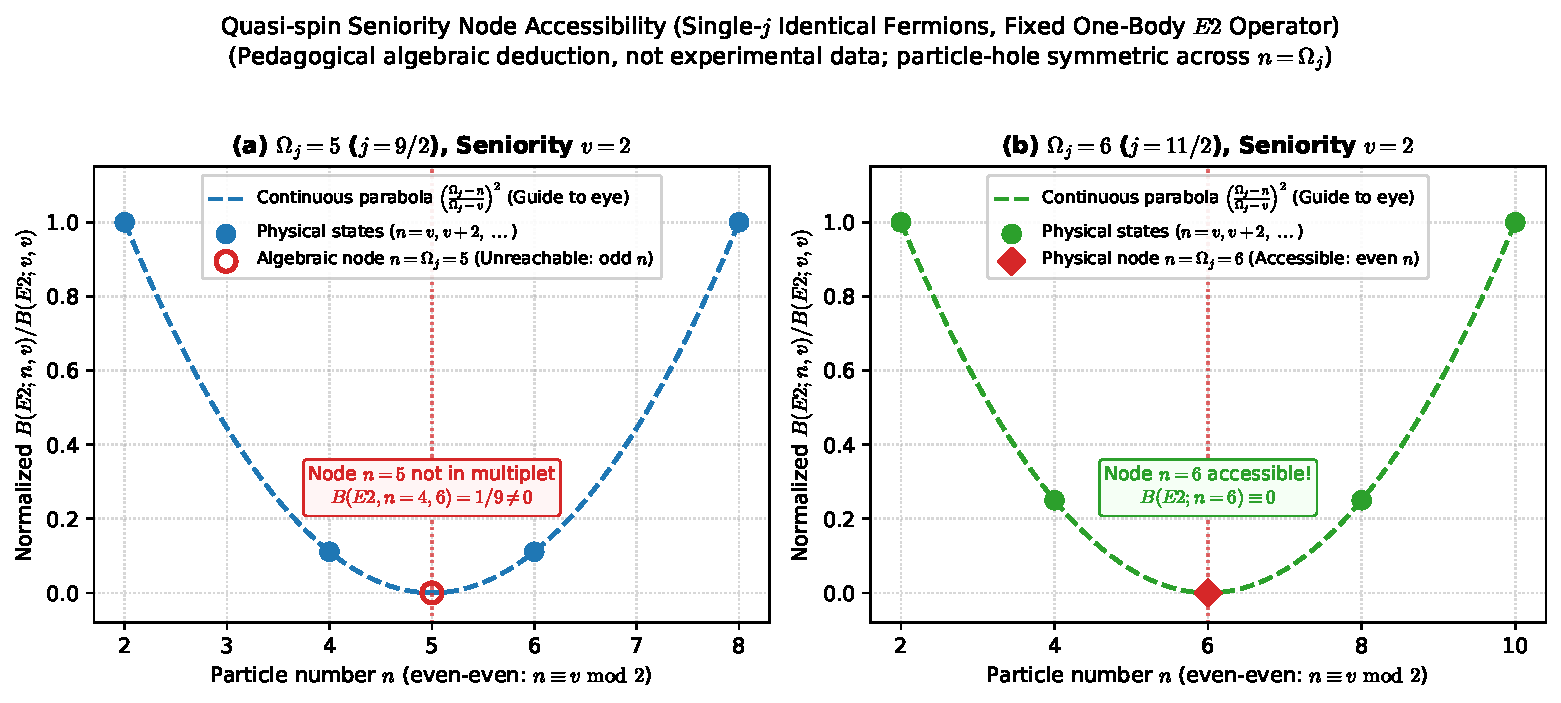
\includegraphics[width=0.88\textwidth]{Img/seniority-node-accessibility.pdf}
\caption[seniority节点的离散占据可达性]{单 $j$ 壳层同种费米子在固定 Seniority $v=2$ 下归一化电四极跃迁强度比 $B(E2; n, v) / B(E2; v, v) = [(\Omega_j - n)/(\Omega_j - v)]^2$ 的离散粒子数可达性对比（教学代数模型推论，非实验寿命预言）。(a) $\Omega_j = 5$（$j=9/2$），偶数 Seniority 家族（$n=2, 4, 6, 8$）永远无法取到奇数代数零点 $n=5$；(b) $\Omega_j = 6$（$j=11/2$），半满点 $n=6$ 为物理允许点，理论上精确击中相消节点。图线展现了跨半满壳 $n = \Omega_j$ 的粒子-空穴对称性。}\label{fig:seniority-node-accessibility}
\end{figure}
\item \textbf{准自旋单态边界（$v = \Omega_j$）：}
若考虑的状态具有最大未配对数 $v = \Omega_j$，则 $S = (\Omega_j - v)/2 = 0$，体系处于准自旋单态（Quasi-Spin Singlet）。此时式~\eqref{eq:4-6-seniority-reduction} 的分母 $\Omega_j - v = 0$ 出现未定义形式。这在物理上意味着准自旋标量态无法通过 $s=1$ 矢量算符实现相同 $S=0$ 态之间的非零耦合（Clebsch-Gordan 系数 $C_{0 0 1 0}^{0 0} \equiv 0$），其物理矩阵元直接由准自旋矢积选择定则决定，并不发生任何物理发散，也不意味着该核素仅存在唯一的量子态。
\item \textbf{算符适用范围规范：}
本推导严格建立在算符属于 $L>0$ 且为偶数的单体电张量算符（在粒子-空穴变换下反演而呈现准自旋矢量性）。该式\textbf{不能无条件推广至单粒子对角期待值或单体标量算符（如粒子数算符 $\hat{N}$ 或电单极算符 $E0$）}，因为标量算符包含非零的准自旋标量成分（$s=0$），其对角期望值具有完全不同的线性斜率。
\item \textbf{跨 Seniority 跃迁（$\Delta v = 2$）与真实多组态混合：}
根据准自旋空间 Wigner-Eckart 定理，张量秩 $s=1$ 的电算符除了连接 $S \to S$（$\Delta v = 0$）外，同样允许在 $|S - S'| = 1$（即改变未配对数 $\Delta v = \pm 2$）的状态之间产生非零矩阵元。对于 $\Delta v = 2$ 跃迁，其矩阵元随粒子数的演化规律与式~\eqref{eq:4-6-seniority-reduction} 截然不同，在半满壳 $n = \Omega_j$ 处并不相消。
在真实原子核中，多 $j$ 壳层组态混合、剩余两体有效电算符以及核芯四极极化微扰会改变相消的精确节点位置与曲线曲率。因此在实际能谱中，纯单 $j$ 壳层的理论零点通常演变为一个平缓或局域下沉的极小值，不能把所有同位素链上的极小化现象都机械当成严格纯单 $j$ 定理。
\end{enumerate}

\paragraph{典型案例剖析与粒子-空穴对称检验：}
考虑锡同位素链中的高自旋异能态。在纯中子 $1h_{11/2}$ 模型中，$\Omega_j=6$，半满节点是该轨道的粒子数 $n=6$。怎样把这一模型占据映射到具体同位素，还需其余价轨道的占据，不能由质量数直接指定。
而在接近中子闭壳的 $^{130}\mathrm{Sn}$（$N=80$）中，中子相当于在 $h_{11/2}$ 壳层容纳了 10 个中子（即 2 个中子空穴，对应 $n=10, v=2$）。将参数代入归约公式~\eqref{eq:4-6-seniority-reduction}：
\begin{equation}\label{eq:4-6-130sn-check}
\frac{\Omega_j - n}{\Omega_j - v} = \frac{6 - 10}{6 - 2} = \frac{-4}{4} = -1 \implies \left( \frac{\Omega_j - n}{\Omega_j - v} \right)^2 = (-1)^2 = 1.
\end{equation}
式~\eqref{eq:4-6-130sn-check} 给出了一个深刻的物理判据：\textbf{$^{130}\mathrm{Sn}$ 并非处于半满相消的零点上}！该式表明，$n=10$（两空穴）的单体 $B(E2)$ 在纯单 $j$ 极限下与 $n=2$（两粒子）的数值严格相同，体现的是粒子-空穴共轭对称性，而非半满相消抑制。
根据核数据评估记录（以 Singh 2001 年在 Nuclear Data Sheets 的采用能级数据快照为例~\cite{singh-2001-nds-130sn-adopted}），$^{130}\mathrm{Sn}$ 测得微秒级半衰期（$T_{1/2} = 1.61(15)\,\mu\mathrm{s}$）的高自旋态实际对应于激发能 $E_x = 2434.79(12)\text{ keV}$ 的 $(10^+)$ 态；该态通过一条低能 $E_\gamma = 96.54(5)\text{ keV}$ 的 $E2$ 射线退激至下方的 $(8^+)$ 态（$E_x = 2338.26(11)\text{ keV}$），采用的反演跃迁强度为 $B(E2) = 0.38(4)\,\text{W.u.}$，总内转换系数高达 $\alpha = 1.829$。需要明确，内转换过程本身的物理效应是增加总跃迁速率（$\lambda_{\mathrm{tot}} = (1+\alpha)\lambda_\gamma$），在给定 $B(E2)$ 与跃迁能量时实际上缩短了激发态的总寿命。该 $(10^+)$ 态之所以表现出微秒级长寿命，其核心物理原因在于跃迁能量极低（仅 $E_\gamma = 96.54\text{ keV}$），使得纯辐射相空间因子 $(E_\gamma)^5$ 受到极强压制，叠合了较小的约化跃迁强度（该 $B(E2) = 0.38(4)\,\text{W.u.}$ 属于核数据评价由寿命与理论转换系数反演导出的导出量，非独立的库仑激发测量）；其长寿命本质上是由低能相空间主导的自旋陷阱效应，绝不能机械看作半满壳相消的产物。而在真实锡同位素链中，从 $^{116}\mathrm{Sn}$ 到 $^{130}\mathrm{Sn}$ 跨越 14 个中子，单粒子能隙与形变相互作用使中子分布于多轨道中，不能简单将代数点 $n=6$ 与特定核素如 $^{122,124}\mathrm{Sn}$ 作刚性的一一对应，真实的极小值位置取决于多轨道占据与剩余相互作用。

\subsection{轴对称形变、K 选择定则与折合阻碍度}\label{sec:4-6-2}

当原子核脱离闭壳区进入稀土区或锕系区时，多核子关联驱动原子核自发产生宏观四极形变。在轴对称形变核的强耦合图景中，内禀参考系具有选定的空间对称轴（体轴 $3$ 轴）。各单核子的角动量投影量子数满足：
\begin{equation}\label{eq:4-6-omega-i-def}
\Omega_i = \Lambda_i + \Sigma_i,
\end{equation}
其中 $\Lambda_i$ 为单粒子轨道角动量投影，$\Sigma_i = \pm 1/2$ 为具有代数符号的内禀自旋投影。多准粒子内禀态在对称轴上的总角动量投影量子数满足代数和：
\begin{equation}\label{eq:4-6-K-def}
K = \sum_i \Omega_i.
\end{equation}
需强调，内禀投影 $K$ 严格不同于实验室系总角动量磁量子数 $M$。即便在静态轴对称形变（$\gamma = 0$）极限下，一旦原子核在转动坐标系中发生旋转，Coriolis 力与粒子-转子耦合依然会引入微扰破缺；因此 $K$ 在真实转动核中始终属于一种近似的好量子数。

当原子核发生多极度为 $\lambda$ 的电磁辐射跃迁时，发射光子在对称轴方向最多只能带走 $\lambda$ 个单位的角动量投影。根据第2.5节的角动量投影代数，从初态 $|I_i K_i\rangle$ 向末态 $|I_f K_f\rangle$ 的电磁跃迁遵守 \textbf{$K$ 选择定则}：
\begin{equation}\label{eq:4-6-K-selection-rule}
\Delta K \equiv |K_i - K_f| \le \lambda.
\end{equation}
当投影改变超过光子多极度时，单K极限中的相应矩阵元为零。这称为K禁戒；真实跃迁需通过混合等机制获得非零振幅。

定义电磁跃迁的 \textbf{$K$ 禁戒度（Degree of $K$-forbiddenness）} 为：
\begin{equation}\label{eq:4-6-forbiddenness-degree}
\nu \equiv \Delta K - \lambda.
\end{equation}
注意：$\nu$ 仅在 $\Delta K > \lambda$ 时定义（即 $\nu \ge 1$）；若 $\nu \le 0$，跃迁为 $K$ 允许跃迁，本概念不适用。

为了定量度量电磁跃迁受到的微观阻碍，实验上首先定义相对于同能量、同多极度的 Weisskopf 单粒子估计值的阻碍因子 $F_W$（Weisskopf Hindrance Factor）~\cite{book-jain-nuclear-isomers}：
\begin{equation}\label{eq:4-6-FW-def}
F_W \equiv \frac{\tau_\gamma(\mathrm{exp})}{\tau_\gamma(W)} = \frac{B_W(\sigma\lambda)}{B(\sigma\lambda; I_i \to I_f)},
\end{equation}
其中实验部分辐射寿命与第5.9节的测量定义严格对齐：若分支比采用包含内转换的总跃迁份额 $b_k^{\mathrm{tot}}$，则 $\tau_\gamma(\mathrm{exp}) = \tau_{\mathrm{exp}} (1 + \alpha_k) / b_k^{\mathrm{tot}}$；若分支比直接采用纯光子发射份额 $b_k^\gamma$，则 $\tau_\gamma(\mathrm{exp}) = \tau_{\mathrm{exp}} / b_k^\gamma$，不可重复乘入 $(1+\alpha)$ 因子。核物理学界引入每个禁戒度单元的平均阻碍率——\textbf{折合阻碍度（Reduced Hindrance per degree of $K$-forbiddenness）} $f_\nu$：
\begin{equation}\label{eq:4-6-fnu-def}
f_\nu \equiv (F_W)^{1/\nu} = \left[ \frac{\tau_\gamma(\mathrm{exp})}{\tau_\gamma(W)} \right]^{1/\nu}.
\end{equation}
式~\eqref{eq:4-6-fnu-def} 是对阻碍因子按禁戒度开根号的定义，适用于 $\nu>0$；它不是准自旋代数给出的普适微观幂律。与同能量、同多极度的Weisskopf估计比较，有助于区分相空间与矩阵元阻碍，但所得数值仍依赖具体支路。$K$ 混合也不限于三轴形状：轴对称平均场之外的Coriolis耦合及残余相互作用同样可能混合不同 $K$ 成分。

\paragraph{经典基准案例：$^{178}\mathrm{Hf}$ 的 $16^+$ 异能态：}
一个经典例子是 $^{178}\mathrm{Hf}$ 的 $K^\pi=16^+$ 异能态。Jain等人的部分能级图给出其能量为2446.1 keV、半衰期约31年；常用指派由质子和中子各一对准粒子构成：~\cite{book-jain-nuclear-isomers}
\begin{equation}\label{eq:4-6-178hf-config}
|\pi^2(7/2^+[404] \otimes 9/2^-[514]) \otimes \nu^2(7/2^-[514] \otimes 9/2^+[624])\rangle_{K=16}.
\end{equation}
同一图中，16$^+$态向 $K=8$ 带的连接涉及很小的能量差。例如到标为 $(13)^-$、2433.3 keV态的图示连接，端点差约12.8 keV；若以最低允许的E3分量讨论，名义禁戒度为 $16-8-3=5$。这项几何计算不能替代该支路多极性、部分光子分支和转换系数的实测或评价。图中的其它低能连接也提示：解释总半衰期必须同时处理低能相空间、内转换及构型阻碍。不能把级联中另一条495-keV光子直接当成16$^+$态的这一出口。

\subsection{三轴非轴对称形变与 K 混合动力学}\label{sec:4-6-3}

当原子核偏离轴对称形变（$\gamma \ne 0$）时，核形状呈现三轴椭球特征。体轴坐标系中的主轴不再具有轴向旋转守恒性，核子总角动量在体轴上的投影 $K$ 不再是严格守恒的好量子数。在正交粒子-转子模型（PRM）基底下，多体态必须展开为不同 $K$ 分量的相干叠加态：
\begin{equation}\label{eq:4-6-K-mixing-expansion}
|\Psi_M^I\rangle = \sum_{K} c_K |I M K\rangle, \quad \sum_K |c_K|^2 = 1.
\end{equation}
注意：若采用第2.5节与附录B中的非正交投影试探基底，展开系数必须通过度规重叠矩阵归一化，式~\eqref{eq:4-6-K-mixing-expansion} 的幺正归一形式严格对应于正交化后的有效粒子-转子基底。

考虑名义上具有高 $K_i$ 的异能态与名义上具有低 $K_f$ 的终态（满足 $\Delta K > \lambda$）。在波函数展开式~\eqref{eq:4-6-K-mixing-expansion} 下，跃迁矩阵元严格由双端混合分量的相干双重求和给出：
\begin{equation}\label{eq:4-6-K-mixed-matrix-element}
\langle \Psi_f^{I_f} || \hat{\mathcal{M}}(\lambda) || \Psi_i^{I_i} \rangle = \sum_{K, K'} c_{K'}^{(f)*} c_K^{(i)} \langle I_f K' || \hat{\mathcal{M}}(\lambda) || I_i K \rangle.
\end{equation}
根据电磁算符选择定则，单粒子矩阵元仅在 $|K - K'| \le \lambda$ 时非零。
\begin{enumerate}
\item \textbf{微弱杂化振幅维持有效阻碍：}
在单一主导退激路径的近似下，跃迁矩阵元取决于初态中掺入的微量低 $K$ 杂质分量（$c_{\mathrm{low}}^{(i)}$）或者终态中掺入的高 $K$ 杂质分量（$c_{\mathrm{high}}^{(f)}$）。由于三轴非轴对称势能曲面的束缚，这些非本征杂化振幅模方通常很小（$|c_K|^2 \ll 1$）。在主导分量占优时，跃迁速率近似标度为 $B(\sigma\lambda) \propto |c_{\mathrm{low}}^{(i)}|^2$ 或 $|c_{\mathrm{high}}^{(f)}|^2$。因此，三轴形变打开了 $K$ 混合通道，但只要非轴对称形变相对适中，杂化振幅的微小性仍然保证跃迁保留可观的阻碍度，绝不意味着三轴形变会使 $K$ 阻碍瞬间消失。
\item \textbf{反向推断非唯一性（反方检验）：}
反过来，若在实验中测得某异能态的折合阻碍度较小（如 $f_\nu < 10$），在科学逻辑上\textbf{严禁直接反推原子核必然存在静态三轴形变}。在真实核系统中，削弱 $K$ 阻碍存在多种平行的微观机制：
\begin{itemize}
\item \textbf{Coriolis 力带混合：} 转动参考系中 Coriolis 算符具有选择定则 $\Delta K = \pm 1$，随自旋升高逐级掺入低 $K$ 成分；
\item \textbf{高激发态密度统计混合：} 在高激发能区，核能级密度剧烈增加，复杂组态相互混合导致纯度下降；
\item \textbf{八极软度：} 空间反射对称破缺与八极振动亦可有效连接不同 $K$ 组态。
\end{itemize}
\end{enumerate}

在过渡核区 $A\approx 190$（Os、Ir、Pt 核素）中，三轴微观动力学展现出极佳的实验室样本。例如在过渡核区 $^{191}\mathrm{Ir}$ 的低能结构研究中，Lukasiak 等人采用粒子-三轴转子模型（PRM）分析了非轴对称势与转动能对低自旋能级及电磁跃迁几率的描述范围~\cite{continuation-g18-lukasiak-1979-191ir-triaxial-rotor}。然而必须指出，三轴粒子-转子模型对低激发集体态的成功描述，不能无条件外推为已从第一性微观上完整解释高自旋长寿命异能态（例如该核区激发能在 $2\text{ MeV}$ 以上的秒级长寿命异能态）；现有理论计算尚未在同组自洽波函数与同一组算符下闭环重现所有高禁戒退激分支比，高自旋异能态的微观组态纯度与三轴动力学响应依然具有明确的外推边界。

\subsection{形状异能态与双峰裂变位垒隧穿}\label{sec:4-6-4}

形状异能态涉及不同形状构型之间受抑制的转换。重核中的经典例子是裂变异能态；形状异能机制并不只限于这种情形。本小节先讨论具有第二形状势阱的裂变例子，其衰变需同时考虑构型重叠、势垒穿透及开放出口。

在超重核与锕系核中，斯楚廷斯基壳修正方法（Strutinsky Shell Correction）揭示：当原子核沿伸长轴拉伸时，液滴模型的光滑势能曲线与单粒子能隙的微观壳修正相叠加，在四极形变空间形成显著的双峰裂变位垒（Double-Humped Fission Barrier）~\cite{book-jain-nuclear-isomers}。其第一势阱对应正常形变基态（ND，$\beta_2 \approx 0.2\text{--}0.25$），内位垒 $V_A$ 隔离了大形变区域，第二势阱对应超形变极小态（SD，典型形变达到 $\beta_2 \approx 0.6$，长短轴比例接近经典的 $2:1$），外位垒 $V_B$ 则通向裂变鞍点。

处于第二极小态的形状异能态面临自发裂变（向外隧穿 $V_B$）与延迟 $\gamma$ 退激（向内隧穿 $V_A$ 回到第一势阱）的统计竞争。根据 WKB 半经典隧穿理论，穿透因子受到位垒作用量积分的指数级压制：
\begin{equation}\label{eq:4-6-WKB-tunneling}
\mathcal{P}_{\mathrm{tunnel}} \propto \exp\left( -\frac{2}{\hbar} \int_{s_{\mathrm{in}}}^{s_{\mathrm{out}}} \sqrt{2 \mathcal{M}(s) \left[ V(s) - E \right]} \, ds \right),
\end{equation}
其中 $\mathcal{M}(s)$ 为依赖于形状坐标的微观惯量参数，$V(s) - E$ 为位垒高度。要由穿透几率得到绝对衰变寿命，理论上还必须给定势阱内的尝试碰撞频率（Attempt Frequency）与前置因子。更重要的是，真实裂变异能态的寿命不仅取决于单维势垒的单纯穿透率，更取决于双峰势垒内复合门态（Doorway States）的共振杂化以及向内穿透辐射 $\gamma$ 退激与向外穿透自发裂变两个分支的竞争比。此外，超形变（$\beta_2 \approx 0.6$）与毫秒级半衰期仅是锕系裂变异能态的特征形态，不能将其作为所有核区全部形状异能态的先验定义。

\paragraph{典型基准发现与概念界限澄清：}
Jain等人的历史回顾叙述了Polikanov等在Dubna重离子实验中发现的延迟裂变：最初观测到约 $10^{-2}$ 秒的活动，后来与 $^{242}\mathrm{Am}$ 约2.2-MeV、14-ms的裂变异能态联系起来，并报告近乎全部经裂变退激。\cite{book-jain-nuclear-isomers} 这里引用的是综述对发现及后续评价的叙述，不能把所有数值倒写成早期一次测量的结果。在比较时还需区分：
\begin{itemize}
\item \textbf{状态身份}：同一核素还有约48-keV、半衰期约141年的低激发异能态；它与上述毫秒裂变态不是同一个态。不同出口及不同形状构型，能使同一核素呈现悬殊的寿命；
\item \textbf{形状共存与形状异能}：低能双 $0^+$ 态可以用于研究形状混合，但“两条 $0^+$ 能级”本身还不等于一个已建立的形状异能机制。需要寿命、E0/E2及模型约束；其中某些受阻转换可形成形状异能态，也不能自动套用锕系双峰裂变势垒。第4.2、4.3节的过渡核比较与这里的裂变例子应按各自观测量连接；
\item \textbf{隧穿阻碍与合成截面的独立性：} 异能态的长寿命仅反映形成之后在势阱内的生存几率，与重离子反应入射道熔合穿透及存活截面完全属于不同物理阶段。
\end{itemize}

\subsection{本节小结与两翼探针接口}\label{sec:4-6-5}

本节系统推演了同核异能态作为多体波函数选择探针的四重物理机制及其数学边界：
\begin{enumerate}
\item \textbf{四机制的电磁标度统一：} 异能态的长寿命根源于辐射跃迁速率式~\eqref{eq:4-6-rate-scaling} 中相空间因子 $(E_\gamma)^{2L+1}$ 的运动学压制（自旋陷阱）、几何代数矩阵元的结构抵消（Seniority 异能态）、空间对称轴角动量投影错位（$K$ 异能态）以及集体势能曲面位垒隧穿压制（形状异能态）。
\item \textbf{Seniority 半满相消：} 在同种核子单 $j$ 壳层中，$\Omega_j=(2j+1)/2$。单体偶多极电算符（$L>0$，如E2）在准自旋空间为秩1张量，$\Delta v=0$归约给出 $(\Omega_j-n)/(\Omega_j-v)$ 因子。其缩放公式要求 $v<\Omega_j$，半满零点还须属于该多重态的允许占据。$v=\Omega_j$须单独用准自旋选择定则处理，不能把公式的零分母解释为物理发散。多轨道混合与有效算符修正会改变实核的简单标度。
\item \textbf{K阻碍与混合：} $f_\nu=(F_W)^{1/\nu}$ 是 $\nu>0$ 时的定义。转移振幅应按初、末两端混合分量相干求和；只有某个小混合振幅主导时，才能近似得到相应模方标度。较小阻碍不能唯一反推三轴形变，Coriolis耦合和其它构型混合也需比较。
\item \textbf{形状异能态与位垒隧穿：} 锕系超形变第二极小态通过厚重位垒隧穿退激，具有 WKB 指数压制特征；必须严格将其与反应生成截面以及低能过渡核的双 $0^+$ 形状共存相区分。
\end{enumerate}

本节所确立的多体波函数选择定则，构筑了通向后续研究的清晰接口：
\begin{itemize}
\item \textbf{对第4.7节与第4.8节：} 弱衰变等待点与异能态热化是相关但不同的问题。例如 $^{130}\mathrm{Cd}$ 的beta衰变参与快过程流强，而 $^{180}\mathrm{Ta}^{\mathrm m}$ 的存活还取决于热网络的桥接与冷却历史。四类异能机制也可能在同一核态中叠加。
\item \textbf{对第5章：} 测量路线取决于寿命、反冲速度与探测响应。在相应敏感窗口内可使用DSAM、RDDS或快定时；更长延迟还可用束流时间结构、反冲输运及延迟符合测量。方法名称本身不规定所有核态都可达到的精度。
\end{itemize}
